\Class{Druid}
{A spirit took me in, when neither of my parents would accept me. Athas provides for those who care for it. We live in a desert simply because no-one cares for the land.}{Sutura, half-elven druid}

Athasian druids are the protectors of Athas' dying landscape. Patient and often unforgiving, they try to preserve and reclaim the barren lands that surround the Tyr region. Well armed with spells and abilities from the Spirits of the Land, they work to bolster Athas' failing ecology.

Often, druids prefer to remain hidden, observing the behavior of creatures and people before passing judgment. Travelers to an oasis are often unaware they are being observed; wanton destruction of the oasis will find themselves under the full fury of the druid and his many abilities.

\SpellcasterTable{The Druid}{.3cm}{
1 & +0 & +2 & +0 & +2 & Animal companion, nature sense, wild empathy & 3 & 1 &  &  &  &  &  &  &  &  \\
2 & +1 & +3 & +0 & +3 & Woodland stride & 4 & 2 &  &  &  &  &  &  &  &  \\
3 & +2 & +3 & +1 & +3 & Trackless step & 4 & 2 & 1 &  &  &  &  &  &  &  \\
4 & +3 & +4 & +1 & +4 & Nature's speech & 5 & 3 & 2 &  &  &  &  &  &  &  \\
5 & +3 & +4 & +1 & +4 & Wild shape (1/day) & 5 & 3 & 2 & 1 &  &  &  &  &  &  \\
6 & +4 & +5 & +2 & +5 & Wild shape (2/day) & 5 & 3 & 3 & 2 &  &  &  &  &  &  \\
7 & +5 & +5 & +2 & +5 & Wild shape (3/day) & 6 & 4 & 3 & 2 & 1 &  &  &  &  &  \\
8 & +6/+1 & +6 & +2 & +6 & Wild shape (Large) & 6 & 4 & 3 & 3 & 2 &  &  &  &  &  \\
9 & +6/+1 & +6 & +3 & +6 & Venom immunity & 6 & 4 & 4 & 3 & 2 & 1 &  &  &  &  \\
10 & +7/+2 & +7 & +3 & +7 & Wild shape (4/day) & 6 & 4 & 4 & 3 & 3 & 2 &  &  &  &  \\
11 & +8/+3 & +7 & +3 & +7 & Wild shape (Tiny) & 6 & 5 & 4 & 4 & 3 & 2 & 1 &  &  &  \\
12 & +9/+4 & +8 & +4 & +8 & Wild shape (plant) & 6 & 5 & 4 & 4 & 3 & 3 & 2 &  &  &  \\
13 & +9/+4 & +8 & +4 & +8 & A thousand faces & 6 & 5 & 5 & 4 & 4 & 3 & 2 & 1 &  &  \\
14 & +10/+5 & +9 & +4 & +9 & Wild shape (5/day) & 6 & 5 & 5 & 4 & 4 & 3 & 3 & 2 &  &  \\
15 & +11/+6/+1 & +9 & +5 & +9 & Timeless body, wild shape (Huge) & 6 & 5 & 5 & 5 & 4 & 4 & 3 & 2 & 1 &  \\
16 & +12/+7/+2 & +10 & +5 & +10 & Wild shape (elemental 1/day) & 6 & 5 & 5 & 5 & 4 & 4 & 3 & 3 & 2 &  \\
17 & +12/+7/+2 & +10 & +5 & +10 &  & 6 & 5 & 5 & 5 & 5 & 4 & 4 & 3 & 2 & 1 \\
18 & +13/+8/+3 & +11 & +6 & +11 & Wild shape (6/day, elemental 2/day) & 6 & 5 & 5 & 5 & 5 & 4 & 4 & 3 & 3 & 2 \\
19 & +14/+9/+4 & +11 & +6 & +11 &  & 6 & 5 & 5 & 5 & 5 & 5 & 4 & 4 & 3 & 2 \\
20 & +15/+10/+5 & +12 & +6 & +12 & Wild shape (elemental 3/day, Huge elemental) & 6 & 5 & 5 & 5 & 5 & 5 & 4 & 4 & 3 & 3}

\begin{figure}[t!]
\centering
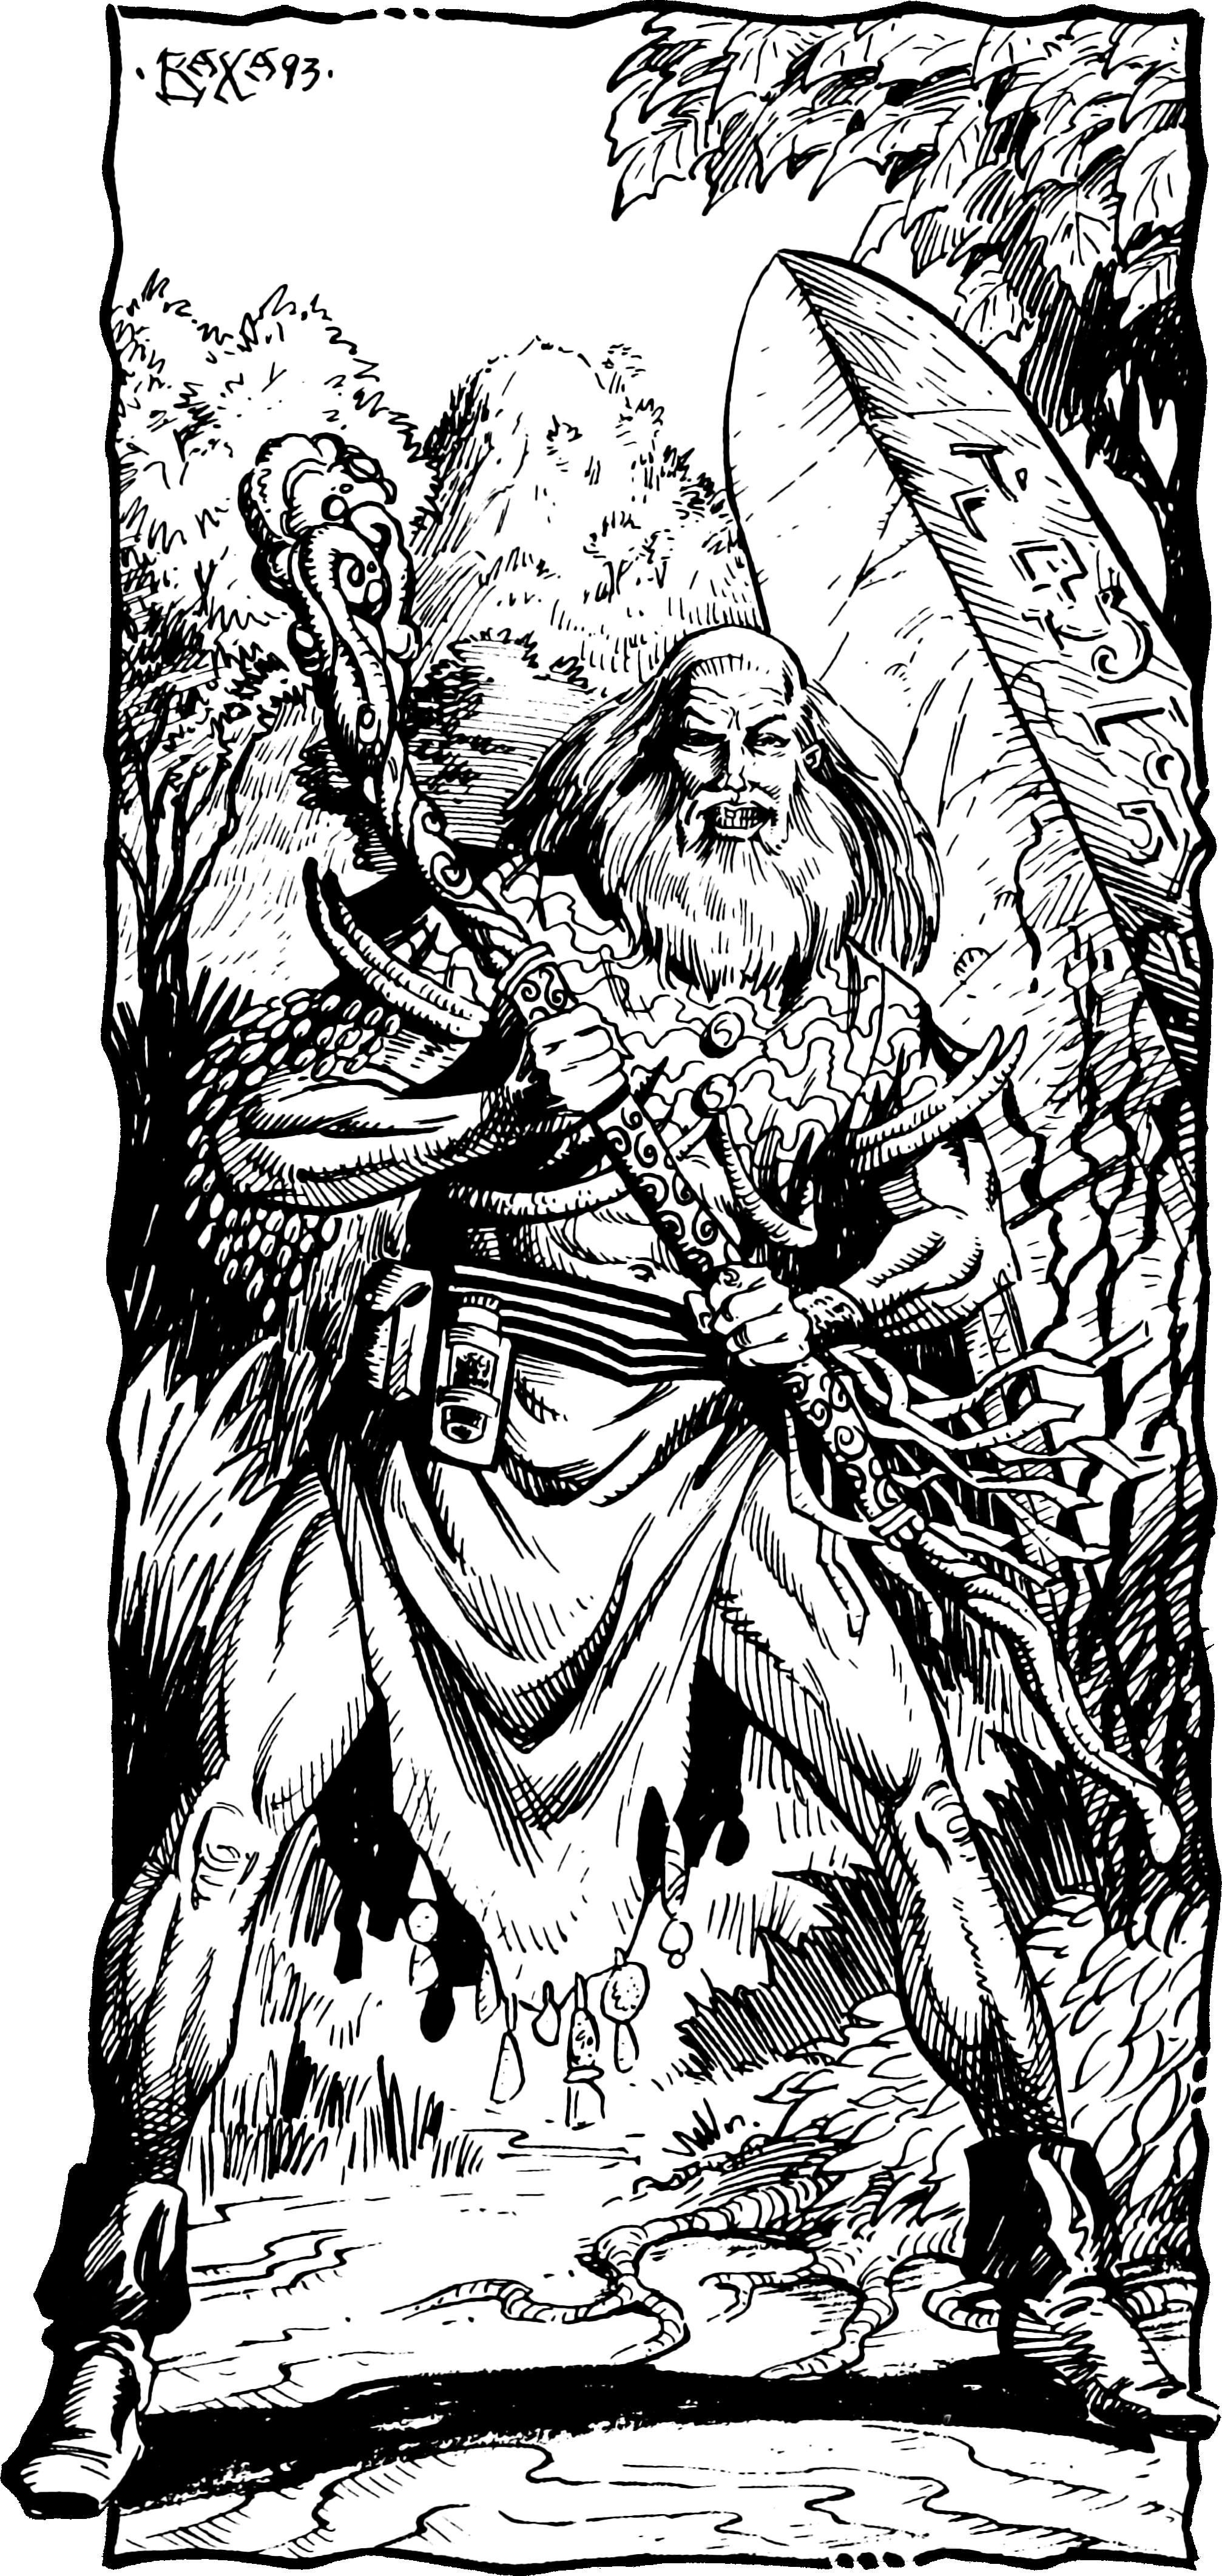
\includegraphics[width=\columnwidth]{images/druid-2.png}
\WOTC
\end{figure}

\subsection{Making a Druid}
Druids cast divine spells through the powers granted them by a spirit of the land. A druid develops a special relationship with the land's spirit. As a druid travels the tablelands, she is recognized by the spirit of the land as a friend. The spirit grants the druid's spells, while the druid protects the land and reinforces the spirit. In addition to spells, druids receive special abilities as they gain in knowledge and power.

\textbf{Races:} Druids come from all races common in the Tablelands, although some have more natural talent than others. Half-elves, with their natural affinity for animals, make good druids. Their often-lonely existence also lends itself well to a lone druid caring for a piece of Athas. Pterrans are often druids, as it follows their Life Path, the Path of the Druid. Aarakocra, muls and Thri-kreen are also good candidates for druids. Halflings druids often hold a position of respect and authority among their tribe. Halfling druids are rarely found outside of the Forest Ridge, though. Half-giants, with their slow wits, make poor druids. Of the savage races, tareks sometimes have druids in their numbers, but rarely do other creatures have the patience or ability to care for a particular piece of Athas.

Druids get along well with most of the races of the Tablelands, provided they respect the natural order of the land. Creatures that kill without need or destroy out of sheer pleasure will find an enemy in the druid.

\textbf{Alignment:} Druids understand the harsh cycle of life and death, of predator and prey, and so one component of their alignment must be neutral. Good druids will tend to help the people they protect, if they serve as protector of a village. They will leave visitors alone, letting them refill their water pouches at no cost, provided there is no abuse. Neutral druids will put the concerns of their guarded lands first, and will not hesitate to punish those that break any rules the druid has determined. Evil druids often rule by fear; some people of the Tablelands prefer the justice of the druid to that of the city-states, even though the druid may be harsh and cruel. The evil druid will often make the villagers work for their protection, helping to plant trees or shrubs, or repair any damage done by a Tyr-storm. Evil druids that guard an oasis or similar geological feature will demand a toll or gift of small bands for the use of their land.

\subsection{Game Rule Information}

\textbf{Alignment:} Any neutral.

\textbf{Hit Die:} d8.

\subsubsection{Class Skills}
\skill{Concentration} (Con), \skill{Craft} (Int), \skill{Handle Animal} (Cha), \skill{Heal} (Wis), \skill{Hide} (Dex), \skill{Knowledge} (nature) (Int), \skill{Listen} (Wis), \skill{Move Silently} (Dex), \skill{Profession} (Wis), \skill{Ride} (Dex), \skill{Spellcraft} (Int), \skill{Spot} (Wis), \skill{Survival} (Wis).

\textbf{Skill Points per Level:} 4 + Int modifier ($\times4$ at 1st level).

\subsubsection{Class Features}

\textbf{Weapon and Armor Proficiency:} Druids are proficient with the following weapons: alak, blowgun, club, dagger, dart, quarterstaff, scimitar, sickle, shortspear, sling, and spear. They are also proficient with all natural attacks (claw, bite, and so forth) of any form they assume with wild shape.

Druids are proficient with light and medium armor but are prohibited from wearing metal armor; thus, they may wear only padded, leather, or hide armor. (A druid may also wear wooden armor that has been altered by the ironwood spell so that it functions as though it were steel. See the ironwood spell description) Druids are proficient with shields (except tower shields) but must use only wooden ones.

A druid who wears prohibited armor or carries a prohibited shield is unable to cast druid spells or use any of her supernatural or spell-like class abilities while doing so and for 24 hours thereafter.

\textbf{Spells:} A druid casts divine spells, which are drawn from the druid spell list. Her alignment may restrict her from casting certain spells opposed to her moral or ethical beliefs; see Chaotic, Evil, Good, and Lawful Spells, below. A druid must choose and prepare her spells in advance (see below).

To prepare or cast a spell, the druid must have a Wisdom score equal to at least 10 + the spell level. The Difficulty Class for a saving throw against a druid's spell is 10 + the spell level + the druid's Wisdom modifier.

Like other spellcasters, a druid can cast only a certain number of spells of each spell level per day. Her base daily spell allotment is given on \tabref{The Druid}. In addition, she receives bonus spells per day if she has a high Wisdom score. She does not have access to any domain spells or granted powers, as a cleric does.

A druid prepares and casts spells the way a cleric does, though she cannot lose a prepared spell to cast a cure spell in its place (but see Spontaneous Casting, below). A druid may prepare and cast any spell on the druid spell list, provided that she can cast spells of  that level, but she must choose which spells to prepare during her daily meditation.

\textbf{Spontaneous Casting:} A druid can channel stored spell energy into summoning spells that she hasn't prepared ahead of time. She can ``lose'' a prepared spell in order to cast any summon nature's ally spell of the same level or lower.

\textbf{Chaotic, Evil, Good, and Lawful Spells:} A druid can't cast spells of an alignment opposed to her own. Spells associated with particular alignments are indicated by the chaos, evil, good, and law descriptors in their spell descriptions.

\textbf{Bonus Languages:} A druid's bonus language options include Sylvan, the language of woodland creatures. This choice is in addition to the bonus languages available to the character because of her race.

A druid also knows Druidic, a secret language known only to druids, which she learns upon becoming a 1st-level druid. Druidic is a free language for a druid; that is, she knows it in addition to her regular allotment of languages and it doesn't take up a language slot. Druids are forbidden to teach this language to nondruids. Druidic has its own alphabet.

\textbf{Animal Companion (Ex):} A druid may begin play with an animal companion selected from the following list: lesser boneclaw, carru, dire rat, eagle, erdlu, jankx, jhakar, kes'trekel, kivit, owl, snake (Small or Medium viper). If the DM's campaign takes place wholly or partly in a silt environment, the DM may add silt spawn to the druid's list of options. This animal is a loyal companion that accompanies the druid on her adventures as appropriate for its kind. 

A 1st-level druid's companion is completely typical for its kind except as noted below. As a druid advances in level, the animal's power increases as shown on the table. If a druid releases her companion from service, she may gain a new one by performing a ceremony requiring 24 uninterrupted hours of prayer. This ceremony can also replace an animal companion that has perished.

A druid of 4th level or higher may select from alternative lists of animals. Should she select an animal companion from one of these alternative lists, the creature gains abilities as if the character's druid level were lower than it actually is. Subtract the value indicated in the appropriate list header from the character's druid level and compare the result with the druid level entry on the table to determine the animal companion's powers. (If this adjustment would reduce the druid's effective level to 0 or lower, she can't have that animal as a companion.)

\textbf{Nature Sense (Ex):} A druid gains a +2 bonus on \skill{Knowledge} (nature) and \skill{Survival} checks.

\textbf{Wild Empathy (Ex):} A druid can improve the attitude of an animal. This ability functions just like a \skill{Diplomacy} check made to improve the attitude of a person. The druid rolls 1d20 and adds her druid level and her Charisma modifier to determine the wild empathy check result. The typical domestic animal has a starting attitude of indifferent, while wild animals are usually unfriendly.

To use wild empathy, the druid and the animal must be able to study each other, which means that they must be within 9 meters of one another under normal conditions. Generally, influencing an animal in this way takes 1 minute but, as with influencing people, it might take more or less time.

A druid can also use this ability to influence a magical beast with an Intelligence score of 1 or 2, but she takes a $-4$ penalty on the check.

\textbf{Woodland Stride (Ex):} Starting at 2nd level, a druid may move through any sort of undergrowth (such as natural thorns, briars, overgrown areas, and similar terrain) at her normal speed and without taking damage or suffering any other impairment. However, thorns, briars, and overgrown areas that have been magically manipulated to impede motion still affect her.

\textbf{Trackless Step (Ex):} Starting at 3rd level, a druid leaves no trail in natural surroundings and cannot be tracked. She may choose to leave a trail if so desired.

\textbf{Nature's Speech (Ex):} Starting at 4th level, a druid become able to speak with animals everywhere, as if under the effects of the speak with animals spell.

\textbf{Wild Shape (Su):} At 5th level, a druid gains the ability to turn herself into any Small or Medium animal and back again once per day. Her options for new forms include all creatures with the animal type. This ability functions like the alternate form special ability, except as noted here. The effect lasts for 1 hour per druid level, or until she changes back. Changing form (to animal or back) is a standard action and doesn't provoke an attack of opportunity. Each time you use wild shape, you regain lost hit points as if you had rested for a night.

Any gear worn or carried by the druid melds into the new form and becomes nonfunctional. When the druid reverts to her true form, any objects previously melded into the new form reappear in the same location on her body that they previously occupied and are once again functional. Any new items worn in the assumed form fall off and land at the druid's feet.

The form chosen must be that of an animal the druid is familiar with.

A druid loses her ability to speak while in animal form because she is limited to the sounds that a normal, untrained animal can make, but she can communicate normally with other animals of the same general grouping as her new form. (The normal sound a wild parrot makes is a squawk, so changing to this form does not permit speech.)

A druid can use this ability more times per day at 6th, 7th, 10th, 14th, and 18th level, as noted on \tabref{The Druid}. In addition, she gains the ability to take the shape of a Large animal at 8th level, a Tiny animal at 11th level, and a Huge animal at 15th level. The new form's Hit Dice can't exceed the character's druid level.

At 12th level, a druid becomes able to use wild shape to change into a plant creature with the same size restrictions as for animal forms. (A druid can't use this ability to take the form of a plant that isn't a creature.)

At 16th level, a druid becomes able to use wild shape to change into a Small, Medium, or Large elemental (air, earth, fire, or water) once per day. These elemental forms are in addition to her normal wild shape usage. In addition to the normal effects of wild shape, the druid gains all the elemental's extraordinary, supernatural, and spell-like abilities. She also gains the elemental's feats for as long as she maintains the wild shape, but she retains her own creature type.

At 18th level, a druid becomes able to assume elemental form twice per day, and at 20th level she can do so three times per day. At 20th level, a druid may use this wild shape ability to change into a Huge elemental.

\textbf{Venom Immunity (Ex):} At 9th level, a druid gains immunity to all poisons.

\textbf{A Thousand Faces (Su):} At 13th level, a druid gains the ability to change her appearance at will, as if using the \spell{disguise self} spell, but only while in her normal form. This affects the druid's body but not her possessions. It is not an illusory effect, but a minor physical alteration of the druid's appearance, within the limits described for the spell.

\textbf{Timeless Body (Ex):} After attaining 15th level, a druid no longer takes ability score penalties for aging and cannot be magically aged. Any penalties she may have already incurred, however, remain in place. Bonuses still accrue, and the druid still dies of old age when her time is up.

\subsubsection{Ex-Druids}
A druid who ceases to revere nature, changes to a prohibited alignment, or teaches the Druidic language to a nondruid loses all spells and druid abilities (including her animal companion, but not including weapon, armor, and shield proficiencies). She cannot thereafter gain levels as a druid until she atones (see the \spell{atonement} spell description).

\subsubsection{The Druid's Animal Companion}
A druid's animal companion is different from a normal animal of its kind in many ways. A druid's animal companion is superior to a normal animal of its kind and has special powers, as described below.

\begin{figure}[b!]
\centering
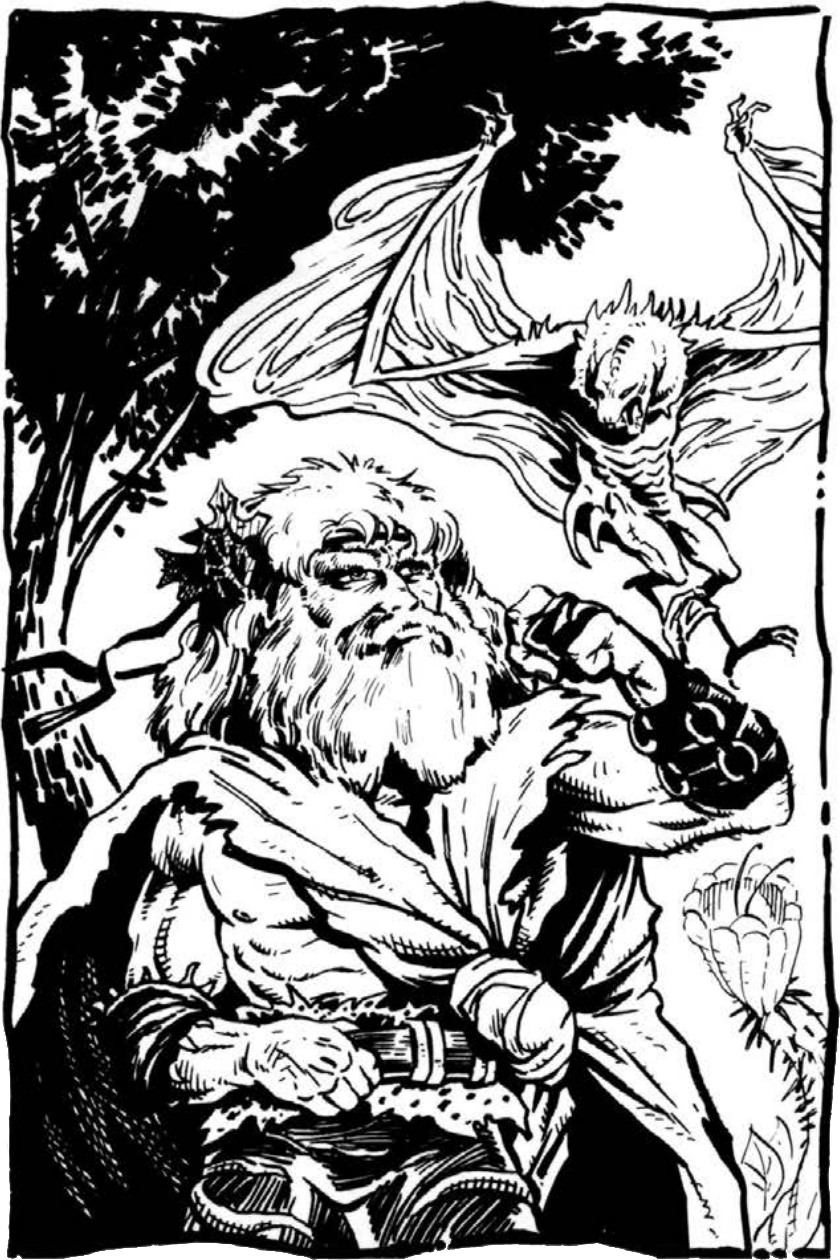
\includegraphics[width=\columnwidth]{images/druid-1.png}
\WOTC
\end{figure}

\Table{}{l Z{.5cm} Z{.8cm} Z{.8cm} Z{.7cm} X}{\tableheader Class Level & \tableheader Bonus HD & \tableheader Natural Armor Adj. &\tableheader  Str/Dex Adj. &\tableheader  Bonus Tricks &\tableheader  Special\\
1st--2nd &&&& 1 & Link, share spells\\
3rd--5th & +2 & +2 & +1 & 2 & Evasion\\
6th--8th & +4 & +4 & +2 & 3 & Devotion\\
9th--11th & +6 & +6 & +3 & 4 & Multiattack\\
12th--14th & +8 & +8 & +4 & 5 &\\
15th--17th & +10 & +10 & +5 & 6 & Improved evasion\\
18th--20th & +12 & +12 & +6 & 7 &}

\textbf{Animal Companion Basics:} Use the base statistics for a creature of the companion's kind, but make the following changes.

\textbf{Class Level:} The character's druid level. The druid's class levels stack with levels of any other classes that are entitled to an animal companion for the purpose of determining the companion's abilities and the alternative lists available to the character.

\textbf{Bonus HD:} Extra eight-sided (d8) Hit Dice, each of which gains a Constitution modifier, as normal. Remember that extra Hit Dice improve the animal companion's base attack and base save bonuses. An animal companion's base attack bonus is the same as that of a druid of a level equal to the animal's HD. An animal companion has good Fortitude and Reflex saves (treat it as a character whose level equals the animal's HD). An animal companion gains additional skill points and feats for bonus HD as normal for advancing a monster's Hit Dice.

\textbf{Natural Armor Adj.:} The number noted here is an improvement to the animal companion's existing natural armor bonus.

\textbf{Str/Dex Adj.:} Add this value to the animal companion's Strength and Dexterity scores.

\textbf{Bonus Tricks:} The value given in this column is the total number of ``bonus'' tricks that the animal knows in addition to any that the druid might choose to teach it (see the \skill{Handle Animal} skill). These bonus tricks don't require any training time or \skill{Handle Animal} checks, and they don't count against the normal limit of tricks known by the animal. The druid selects these bonus tricks, and once selected, they can't be changed.

\textbf{Link (Ex):} A druid can handle her animal companion as a free action, or push it as a move action, even if she doesn't have any ranks in the Handle Animal skill. The druid gains a +4 circumstance bonus on all wild empathy checks and Handle Animal checks made regarding an animal companion.

\textbf{Share Spells (Ex):} At the druid's option, she may have any spell (but not any spell-like ability) she casts upon herself also affect her animal companion. The animal companion must be within 1.5 meter of her at the time of casting to receive the benefit. If the spell or effect has a duration other than instantaneous, it stops affecting the animal companion if the companion moves farther than 1.5 meter away and will not affect the animal again, even if it returns to the druid before the duration expires.

Additionally, the druid may cast a spell with a target of ``You'' on her animal companion (as a touch range spell) instead of on herself. A druid and her animal companion can share spells even if the spells normally do not affect creatures of the companion's type (animal).

\textbf{Evasion (Ex):} If an animal companion is subjected to an attack that normally allows a Reflex saving throw for half damage, it takes no damage if it makes a successful saving throw.

\textbf{Devotion (Ex):} An animal companion gains a +4 morale bonus on Will saves against enchantment spells and effects.

\textbf{Multiattack:} An animal companion gains \feat{Multiattack} as a bonus feat if it has three or more natural attacks and does not already have that feat. If it does not have the requisite three or more natural attacks, the animal companion instead gains a second attack with its primary natural weapon, albeit at a $-5$ penalty.

\textbf{Improved Evasion (Ex):} When subjected to an attack that normally allows a Reflex saving throw for half damage, an animal companion takes no damage if it makes a successful saving throw and only half damage if the saving throw fails.

\subsubsection{Alternative Animal Companions}
A druid of sufficiently high level can select her animal companion from one of the following lists, applying the indicated adjustment to the druid's level (in parentheses) for purposes of determining the companion's characteristics and special abilities.

Some animals are only available in certain environments. The animals available only in an aquatic environment, such as the Last Sea, are marked with $\dagger$. The animals available only in a silt environment, such as the Sea of Silt, are marked with $\diamond$.

\Table{}{X X}{
\multicolumn{2}{c}{\tableheader\footnotesize 4th Level or Higher (Level $-3$)}\\
Carru, bull (6HD) & Leopard \\
Cheetah & Lizard, giant \\
Crodlu & Lizard, monitor\\
Crodlu, heavy & Rasclinn\\
Dire bat & Athasian shark$^\dagger$\\
Erdland & Snake, constrictor\\
Jhakar, Medium (6HD) & Snake, viper (Large)\\
Kluzd & }

\Table{}{X X}{
\multicolumn{2}{c}{\tableheader\footnotesize 7th Level or Higher (Level $-6$)}\\
Crodlu, heavy warmount & Puddingfish$^\dagger$ \\
Inix & Lion\\
Kalin & Lizard, subterranean\\
Kluzd (7HD) & Snake, viper (Huge)\\
Lirr & Takis\\
Pterrax & Tiger}

\Table{}{X X}{
\multicolumn{2}{c}{\tableheader\footnotesize 10th Level or Higher (Level $-9$)}\\
Cha'thrang & Lizard, minotaur\\
Dire lion & Athasian shark (Huge)$^\dagger$ \\
Hatori & Snake, giant constrictor}

\Table{}{X X}{
\multicolumn{2}{c}{\tableheader\footnotesize 13th Level or Higher (Level $-12$)}\\
Lirr, large (11HD) & Athasian sloth\\
Ruktoi$^\diamond$ & }

\Table{}{X X}{
\multicolumn{2}{c}{\tableheader\footnotesize 16th Level or Higher (Level $-15$)}\\
Dire Athasian shark$^\dagger$ & Silt Horror, white$^\diamond$\\
Dire tiger&Slimahacc\\
Hatori, gargantuan (17HD) &}

\subsection{Playing a Druid}
You are a humanoid servant devoted to Athas and all of its elements equally. As a guardian, tender, warrior, and sometimes assassin, you further the cause of nature and help to make Athas verdant again.

You, like nature itself is neutral. You see the balance of all things. You know that every living creature is part of the food chain, and birth and death are the natural order of life. This is one of the reasons druids harbor such intense hatred for the defilers. Their magic of decay lies outside the normal cycle of life. Matter should not be destroyed, but converted to a form that will eventually return to the earth. Defiling magic destroys that which should never be destroyed, and its practice is an abomination to druids.

\subsubsection{Religion}
A druid is an individual who has devoted themselves to the balance of nature on Athas, and in particular someone who has sought out or been chosen by one of the few living spirits left in the barren land, protecting and nurturing them and the natural balance they represent.

Individual druids do not necessarily recognize one another as kin or as brothers in a religion; each conducts their affairs as they see fit in their quest to restore the balance of nature and protect their spirit's lands. Most druids recognize the various spirits as a manifestation of Athas itself, though some few more primitive or uncultured individuals or groups may believe the spirit to be a god and treat it as such.

\subsubsection{Other Classes}
Druids get along with most classes, though they despise wizards. Magic is the cause of Athas' current state, so say the druids, and while they may tolerate preservers for a short while, defilers are slain on sight. Templars are usually not welcomed by druids, as the templar is responsible for a city that encroaches on nature, and templars serve the sorcerer-kings, Athas' most powerful magic users. Elemental clerics are well received by druids, as they often share the same goals. Druids are usually at odds with paraelemental clerics, though. The paraelement proliferation on Athas is usually at the land's expense, destroying what the druid tries to accomplish.

Rangers are probably the druid's best allies. They often share the same goals, and the druid may even call upon the ranger for help in controlling a species that has become problematic or detrimental to an area. However, the ranger and the druid may sometimes be at odds, if the ranger is determined to eradicate his favored enemy while the druid seeks to protect that particular species.

\subsubsection{Combat}
Your ability to summon creatures and to turn into them is your primary weapons. Consider using them to aid your companions in flanking maneuvers, or better yet to harass enemy spellcasters (many of whom are easy to hit), especially if they are defilers. Few foes are prepared for an opponent who can call such potent beings to service, so you've also got the advantage of surprise.

Though somewhat skilled at both combat and spellcasting, you are more suited to guerrilla warfare---tracking enemies to their lair ambushing them while they sleep, or engaging in other sue surreptitious tactics. With woodland stride and trackless step, you can usually escape through the wilderness before your enemies know what hit them.

\subsubsection{Advancement}

You profit most from remaining a druid thought your advancement, so that your animal companion and wild shape continue to improve as you gain levels. If you do multiclass, a level of barbarian is an excellent choice; the benefits it grants to combat and movement regardless of when you take that 1st level.

During their time of wandering, a young druid learns about the world, its ecology, the balance of nature and the ways of its creatures. After a few years of peregrination, most druids decide to settle in order to watch over a specific patch of land lands, watching over them and protecting them, and straighten their bond with a Spirit of the Land. Such druids become \class{Grove Masters}.

\subsection{Starting Packages}
\subsubsection{The Beastmaster}

Half-Elf Druid

\textbf{Ability Scores:} Str 10, Dex 15, Con 12, Int 8, Wis 15, Cha 12.

\textbf{Skills:} \skill{Handle Animal}, \skill{Hide}, \skill{Survival}.

\textbf{Languages:} Common, Elven.

\textbf{Feat:} \feat{Animal Affinity}.

\textbf{Weapons:} Longspear (1d8/$\times$3)

Sling with 20 bullets (1d4, 15 m).

\textbf{Armor:} Hide (+3 AC).

\textbf{Gear:} Spell component pouch, standard adventurer's kit, 20 cp.

\textbf{Class Features:} Jankx animal companion.

\textbf{Spells Prepared:} 1st---\spell{cure light wounds}, \spell{speak with animals}; 0---\spell{cure minor wounds} (2), \spell{defiler scent}.

\subsubsection{The Defiler Hunter}

Human Druid

\textbf{Ability Scores:} Str 13, Dex 14, Con 12, Int 10, Wis 15, Cha 8.

\textbf{Skills:} \skill{Concentration}, \skill{Hide}, \skill{Listen}, \skill{Move Silently}, \skill{Spot}, \skill{Survival}.

\textbf{Languages:} Common

\textbf{Feat:} \feat{Defender of the Land}, \feat{Track}.

\textbf{Weapons:} Spear (1d8/$\times$3, 6m)

Sling with 20 bullets (1d4, 15 m).

\textbf{Armor:} Hide (+3 AC).

\textbf{Gear:} Spell component pouch, standard adventurer's kit, 20 cp.

\textbf{Class Features:} Jhakar animal companion.

\textbf{Spells Prepared:} 1st---\spell{backlash}, \spell{longstrider};\hskip10pt 0---\spell{cure minor wounds}, \spell{defiler scent} (2).

\subsubsection{The Warden}

Pterran Druid

\textbf{Ability Scores:} Str 8, Dex 11, Con 14, Int 10, Wis 17, Cha 14.

\textbf{Skills:} \skill{Hide}, \skill{Knowledge} (nature), \skill{Move Silently}, \skill{Spot}, \skill{Survival}.

\textbf{Languages:} Saurian.

\textbf{Feat:} \feat{Spell Focus} (conjuration).

\textbf{Weapons:} Alak (1d6/$\times$3)

Blowgun with 20 needles (1, 3 m).

\textbf{Armor:} Leather (+2 AC), light wooden shield (+1 AC).

\textbf{Gear:} Spell component pouch, standard adventurer's kit, 20 cp.

\textbf{Class Features:} Lesser boneclaw animal companion.

\textbf{Spells Prepared:} 1st---\spell{entangle}, \spell{plant renewal}; 0---\spell{defiler scent}, \spell{detect magic}, \spell{nurturing seeds}.

\subsection{Druids on Athas}
\Quote{The druids are no longer hunted in force by the sorcerer-kings. The kings believe there simply aren't enough left to threaten them. But the templars, and even some elves I know, have been well rewarded for delivering the heads of wasteland druids.}{Jurgan, Urikite earth cleric}

Perhaps the only thing rarer to see in Athas than a wizard is a druid. After centuries of persecution, they were forced to either die in the hands of the agents of the sorcerer-monarchs, or to watch their beloved land wither and die before their eyes.

Because of that, druids are usually loners and avert to social interaction. They live off the land, within the land, and they have sacrificed their entire lives for the land, very little besides it occupies the mind of a druid.

\subsubsection{Daily Life}

A druid adventures to learn about Athas, to protect nature, and to further his own aims. Druids usually spend their days in contemplation of nature, and tending their lands; one may watch over a particular stretch of open desert, another may protect a belt of scrub grass within it, while still another might watch over a small oasis that borders on both, always hidden and always watching.

The Athasian druid is a wanderer who hunts down a powerful defiler that has despoiled the wastes, or a visionary who tends the land and teaches the local population how to live in harmony with their surroundings. The Athasian druid fights for an almost lost cause, and it matters not if that cause is revenge himself against those who destroyed his land and friends or a ceaseless desire to bring green and hope to Athas.

\subsubsection{Notables}

Druids very rarely become famous, since they usually avoid social interaction combined the fact that it might put their lives at risk since usually sorcerer-kings and defiler usually put a reward for the head of a notorious or troublesome druid. A legend claim that Mearedes the druidess came to the island of Shault when its forest was all but dead and she managed to nurture it back to its vibrant health.

\subsubsection{Organizations}

Ever since the Eradication, an anti-druidic jihad led by sorcerer-kings more than 1,500 years ago, no specific druidic organization exists, although some form temporary alliances with Veiled Alliance members from time to time. Legends say that the druids who remained after the Eradication gathered on a high mesa somewhere in the northern Tablelands. It was there they decided that they should scatter to the most remote reaches and farthest regions of Athas, there to bide their time, waiting for the day when they were powerful enough to challenge the sorcerer-kings again. This was a long time ago, and the druids have yet to return to the cities of the defilers. Some say that they will never return and that their seclusion and isolation have destroyed whatever power they once wielded as a circle. Others say that the druid's long wait is indicative of their cunning, and that their plan is to insure that the next confrontation with the kings won't end in defeat.

\subsubsection{NPC Reactions}

Druids are natural loners, and usually avoid social interactions unless they have to. In such cases, those who are directly benefited from the druid's work of tending the land begin two steps nearer helpful, while defilers and evil paraelemental clerics begin two steps nearer hostile.

\subsubsection{Druid Lore}

Characters with ranks in \skill{Knowledge} (nature) can research druids to learn more about them. When a character makes a skill check, read or paraphrase the following, including the information from lower DCs.

\textbf{DC 10:} Druids devote themselves to the land, drawing off their power straight from Athas itself.

\textbf{DC 15:} Druids from a mystical connection to mysterious beings known as Spirits of the Land. They hate all defilers and those who abuse the land.

\textbf{DC 20:} Druids are masters of the forces of nature, being able to transform into the creatures that dwell in their lands, and some even learn to counter the destruction of defilement.
